\data{02/03/2026}
\section{Alcune note iniziali}
Il primo esame è composto da 2 prove parziali, ciascuna  vale 25\% prova iniziale + 25\% prova finale. Il restante 50\% è riservato ad un progetto individuale $$25\%PI+25\%PF+50\% P$$
Gli altri appelli (2,3,4 e 5) sono $100\%$ esame scritto (no progetto).

Il corso finisce circa a metà maggio. Il primo appello è all'inizio di giugno. Il progetto viene assegnato circa a metà del semestre e comprende una relazione. Il libro di testo è di \textit{Aanon Brandley \& Zohan Manna} che usa un linguaggio di programmazione ideale che si chiama $\pi$ che è simile al C ma semplificato. \textbf{Rust} sarà presente in questo corso. Verus (della Microsoft) e Why (Rust Belt). La verifica Rust (colleghi di Parigi che insegnano codifica Rust).
\section{Una panoramica sulla verifica di programmi}Floyd e Hoare furono i pionieri di questa teoria alla fine degli anni 60. Il limite fondamentale per la verifica automatica di programmi resta sempre lo stesso: non possiamo creare un verificatore universale che decida la correttezza semantica per programmi arbitrari\cite{rice-app}. Questa condizione viene garantita dal \cref{thm:Rice}.
\begin{theorem}[di Rice]
	Il teorema di Rice stabilisce che tutte le proprietà non banali delle funzioni calcolabili da programmi (tranne quelle sempre vere o sempre false) sono indecidibili, ovvero non esiste un algoritmo generale che, dato un programma, possa determinare automaticamente se soddisfa tale proprietà.\cite{rice}
	\label{thm:Rice}
\end{theorem}
In pratica, si aggirano questi limiti con approssimazioni, analisi statiche conservative, o restrizioni sul dominio (es. programmi finiti o lineari), ma la verifica totale resta impossibile \cite{rice-app}.
Esistono degli strumenti per effettuare quella che viene chiamata \textit{analisi statica} per fare la dimostrazione di correttezza di un programma a partire dal suo codice sorgente in modo quasi totalmente meccanico. Ci sono tre tecniche fondamentali che andremo a studiare in questa prima parte del corso:
\begin{enumerate}
	\bitem{La specifica}specificazione di un programma. Quello che un programma deve fare (caricare qualcosa su un sito, ordinare un array) viene descritto con formule in \textbf{logica del $1^\circ$ ordine}. Ad esempio per dire che un array è ordinato tra l'indice $l$ e l'indice $u$ bisogna dire $$sorted(a,l,u)\equiv\forall i\forall j\colon l\le i\le j\le u \implies a[i]\le a[j] $$ La logica composizionale da sola non è sufficientemente espressiva. Avremo bisogno di scrivere per ogni funzione\footnote{ogni programma può essere visto come una collezione di funzioni.} di un programma bisogna specificare:
	\begin{enumerate}
		\bitem{Pre-condizione}  è un qualcosa che si assume vero prima che inizi la computazione della funzione. Contiene anche ciò che la funzione assume per poter lavorare. Descrive lo stato del programma prima dell'esecuzione della funzione. Utilizzeremo la parola chiave \textit{``requires''} cioè ciò che la funzione richiede prima della sua esecuzione.
		\bitem{Post-condizione} ciò che vale dopo l'esecuzione della funzione. Descrive lo stato del programma dopo la computazione della funzione. Utilizzeremo la parola chiave \textit{``ensures''} cioè ciò che la funzione assicura dopo la sua esecuzione.
	\end{enumerate}
	L'esecuzione di una funzione modifica lo stato di un programma. 
	
	Le annotazioni (la categoria generale a cui appartengono le pre-condizioni e le post-condizioni) sono formule incorporate nel codice e si distinguono nel modo seguente:
	\begin{itemize}
		\bitem{pre-condizioni}  formule che devono valere prima dell'esecuzione della funzione;
		\bitem{post-condizioni} formule che devono valere dopo l'esecuzione della funzione;
		\bitem{asserzioni} formule contenute nel corpo della funzione che devono valere in quel punto nel codice.
	\end{itemize}
	
	Le annotazioni sono riconoscibili dentro il codice perché riportano la chiocciola @L\footnote{L è una label.}: F\footnote{formula di logica del primo ordine che deve essere vera nello stato del programma.}
	Quindi da un programma 
	\begin{lstlisting}
		<type> foo(<type_1> param_1 ... <type_n> param_n)
		{
			<block_1>
			<block_2>
			return(  )  
		}
	\end{lstlisting}
	si ottiene un programma annotato
	\begin{lstlisting}
		@pre: F
		@post: G
		<type> foo(<type_1> param_1 ... <type_n> param_n)
		{
			<block_1>
			@L: H 
			<block_2>
			return(  )  
		}
	\end{lstlisting}
	C'è una branca dell'informatica che studia come generare automaticamente le annotazioni. In questo corso non riusciamo a vedere questa parte e le scriveremo sempre manualmente. La formula \texttt{H} deve essere vera nello \textbf{stato del programma} a quel punto (linea interessata da \texttt{@L: H}).
	\paragraph{Stato del programma} È definito dall'indirizzo di programma nel PC\footnote{program counter.} e le variabili del programma (ad esempio $x:int,y:int,\, i:int,\, j:int,\, a:int[]$). Lo stato è una fotografia della memoria nell'esecuzione. 
	\begin{lstlisting}
		PC = 0010011
		x = 5
		y = 0
		j = -2 
		a = [0,0,3,0,17,-1]
	\end{lstlisting}
	Quindi lo stato del programma può essere visto come un assegnamento di valori del tipo richiesto al PC e a ogni variabile (parametri) del programma.
	
	\begin{lstlisting}
		@pre: F
		@post: G
		<type> foo(<type_1> param_1, <type_n> param_n)
		{
			<block_1>
			@L: H
			<block_2>
			return(  )  
		}
	\end{lstlisting}
	Se la funzione foo viene chiamata con $ \textit{foo}(a,0,16)$ vuol dire che $param_1 = a$, $param_2 = 0$, $param_3 = 16$.  I \textbf{parametri} (o \textit{``parametri formali''}) sono quelli che definiscono la funzione, gli \textbf{argomenti} (o \textit{``parametri attuali''}) sono quelli della chiamata di funzione. Un parametro può essere passato \textbf{per valore} (la funzione non può modificarlo; tutti i parametri sono passati per valore nel linguaggio \texttt{pi}) o \textbf{per riferimento} (il valore può essere modificato dalla funzione).
	\bitem{Metodo delle asserzioni induttive} È un metodo per dimostrare \textbf{proprietà di correttezza parziale} (o in generale ``\textit{safety}'') ovvero che il programma non va in stato d'errore. Se un'asserzione è vera nello stato $0$, e nello stato $n$, allora deve essere anche nello stato $n+1$. Questa è solo l'intuizione dell'induzione ben fondata utilizzata nel metodo delle asserzioni induttive. 
	\begin{itemize}
		
		\bitem{Funzione parzialmente corretta}una funzione è \textit{parzialmente corretta} se per ogni ingresso che soddisfa la pre-condizione, se la funzione termina, allora l'uscita soddisfa la post-condizione\footnote{Nota: stiamo parlando degli ingressi e uscite delle funzioni di un programma, non dell'ingresso e dell'uscita di un programma.}. Si dice \textit{``parzialmente''} perché si ammette la terminazione della funzione. Il termine \textit{``corretta''} viene usato perché pre e post-condizione sono valide. 
		
		\bitem{Funzione totalmente corretta}una funzione è \textit{totalmente corretta} se per ogni ingresso che soddisfa la pre-condizione, la funzione termina e l'uscita soddisfa la post-condizione.
	\end{itemize}
	\bitem{Metodo delle funzioni d'ordine} viene usata sui valori e sulla ricorsione. Viene usata per la totale correttezza, quindi per dimostrare la terminazione. \textbf{Funzione d'ordine} perché tipicamente la terminazione viene dimostrata dando una funzione definita come un'espressione costruita sulle variabili di un programma che mappa l'espressione ad un valore, in un dominio, con un ordinamento ben fondato (per esempio i numeri naturali). Si dimostra che, ad ogni chiamata ricorsiva o ad ogni iterazione/chiamata ricorsiva del ciclo, l'espressione diventa più piccola. In un ordinamento ben fondato, per esempio su i numeri naturali, se si definisce una funzione su un dominio con ordinamento ben fondato in termini di variabili di programma e si mostra che ad ogni iterazione l'espressione diventa più piccola, siccome lo zero è il fondo dell'ordinamento ben fondato, non potrà scendere all'infinito e quindi il ciclo terminerà.
\end{enumerate}
Le specifiche non sono completamente automatizzate mentre i metodi delle asserzioni induttive e delle funzioni d'ordine sì.

\begin{figure}[thbp]
	\centering
	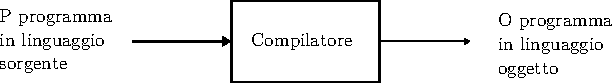
\includegraphics{compilatore}
	\caption{compilatore.}
	\label{fig:compilatore}
\end{figure}

In un linguaggio di programmazione, un compilatore (\cref{fig:compilatore}) prende in ingresso un programma $P$ in un linguaggio sorgente e restituisce un programma $O$ nel linguaggio oggetto. 
\begin{figure}[tbph]
	\centering
	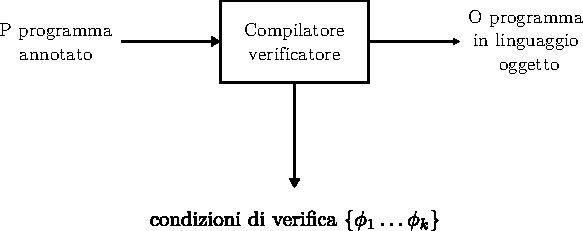
\includegraphics[width=0.7\linewidth]{compilatore-verificatore}
	\caption{compilatore verificatore.}
	\label{fig:compilatore-verificatore}
\end{figure}

Un compilatore verificatore (\cref{fig:compilatore-verificatore}) prende in ingresso un programma $P$ annotato (pre-condizioni, post-condizioni, asserzioni e programma nel linguaggio sorgente di prima) e restituisce in uscita: 
\begin{enumerate}
	\item un programma $O$ nel linguaggio oggetto del compilatore precedente;
	\item delle formule $\{\phi_1\dots\phi_k\}$ dette \textbf{condizioni di verifica} che sono formule la cui validità assicura che il programma è parzialmente corretto se si usa solo il metodo delle asserzioni induttive e totalmente corretto se si usa anche il metodo delle funzioni d'ordine. Il metodo delle asserzioni induttive e il metodo delle funzioni d'ordine sono \textit{pienamente automatizzabili}, mentre la specifica no.
\end{enumerate}
Questi compilatori implementano i metodi delle asserzioni induttive e delle funzioni d'ordine. Purtroppo non sono completamente automatizzabili come in \cref{fig:dimostratore-teoremi-ideale} per il \cref{thm:Rice}.
\begin{figure}[tbph]
	\centering
	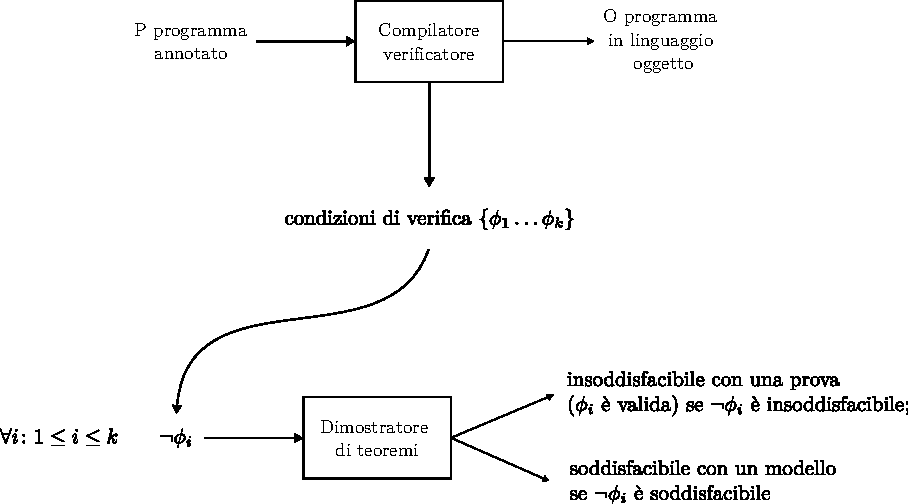
\includegraphics[width=.8\linewidth]{dimostratore-teoremi-ideale}
	\caption{dimostratore di teoremi nel caso ideale.}
	\label{fig:dimostratore-teoremi-ideale}
\end{figure}

$\forall i\ 1\le i\le k$ si ha che $\neg \phi_i$ in un dimostratore di teoremi che sia una \textbf{procedura di decisione} risponde con:
\begin{itemize}
	\item insoddisfacibile con una prova ($\phi_i$ è valida) se $\neg\phi_i$ è insoddisfacibile;
	\item soddisfacibile con un modello se $\neg\phi_i$ è soddisfacibile.
\end{itemize}

\begin{figure}[tbph]
	\centering
	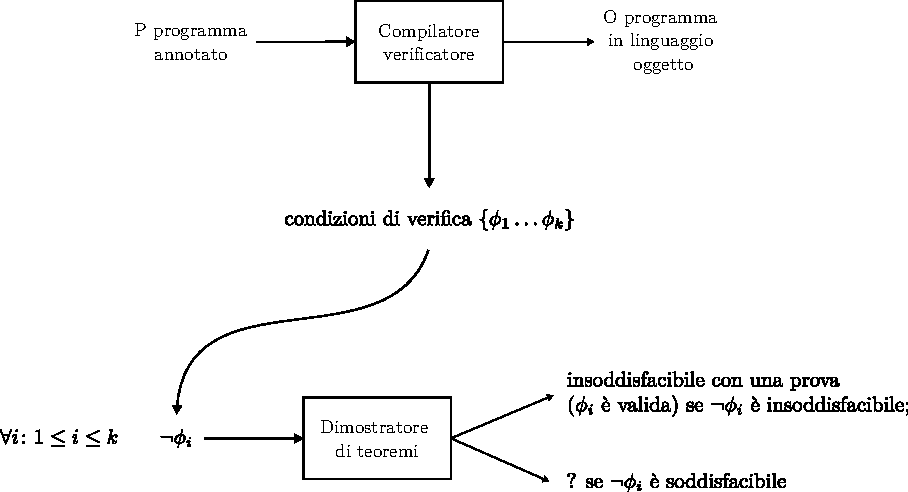
\includegraphics[width=.8\linewidth]{dimostratore-teoremi-semidecidibile}
	\caption{il dimostratore di teoremi nella logica del $1^\circ$ è semidecidibile.}
	\label{fig:dimostratore-teoremi-semidecidibile}
\end{figure}

Nella logica del $1^\circ$ ordine, l'insoddisfacibilità o equivalentemente la validità è solo semi-decidibile. 

Un dimostratore di teoremi che prende in ingresso $\neg\phi_i$ restituisce: 
\begin{itemize}
	\item insoddisfacibile\footnote{significa che è sempre falsa.} con prova se $\exists i.\neg\phi_i$ è insoddisfacibile ($\forall i.\phi_i$ è valida\footnote{è sempre vera.});
	\item ? se $\neg\phi_i $ è soddisfacibile. 
\end{itemize}

Avendo a disposizione una \textbf{procedura di decisione}, vorremmo che il dimostratore rispondesse:
\begin{itemize}
	\item insoddisfacibile con prova se $\exists i. \neg\phi_i$ è insoddisfacibile;
	\item soddisfacibile con un modello se $\neg\phi_i$ è soddisfacibile.
\end{itemize}

Se $\neg\phi_i$ è soddisfacibile, vuol dire che $\phi_i$, che è una formula restituita dal compilatore-verificatore, è in-valida (cioè non valida). Avere un modello permette di ricostruire, in fase di debugging, lo stato di non validità del programma quando $\phi_i$ è in-valida.
